\section{Reconstruction and Samples from the Moving-MNIST Dataset}
\label{app:mnist_visual}


\subsection{Reconstructions}
\begin{center}

    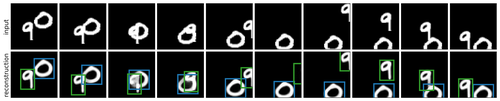
\includegraphics[width=\linewidth]{figures/SQAIR/mnist_rec/000047.png}
    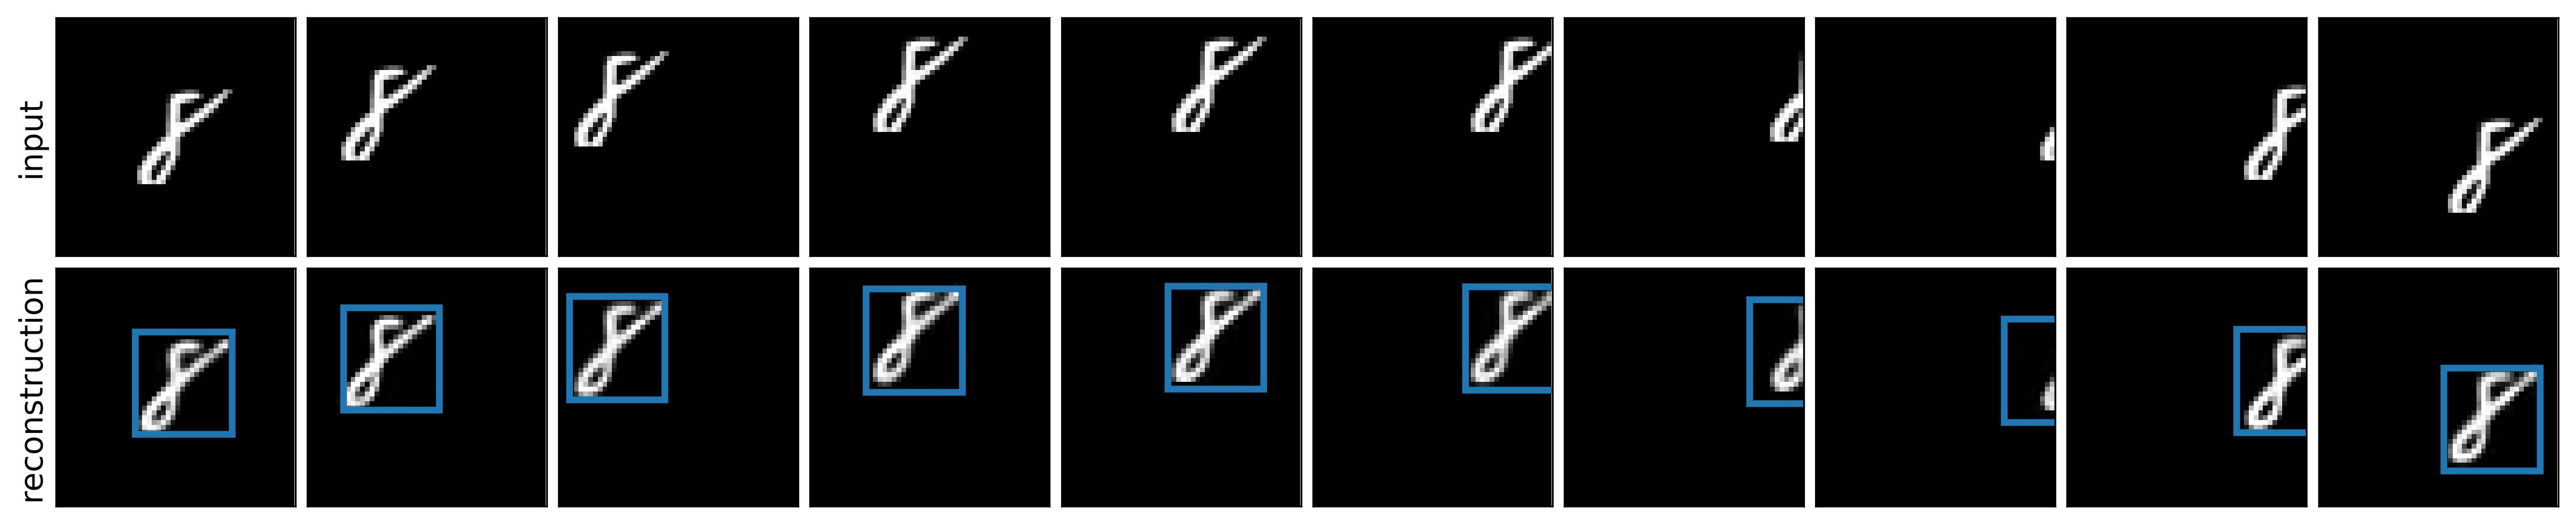
\includegraphics[width=\linewidth]{figures/SQAIR/mnist_rec/000050.png}
    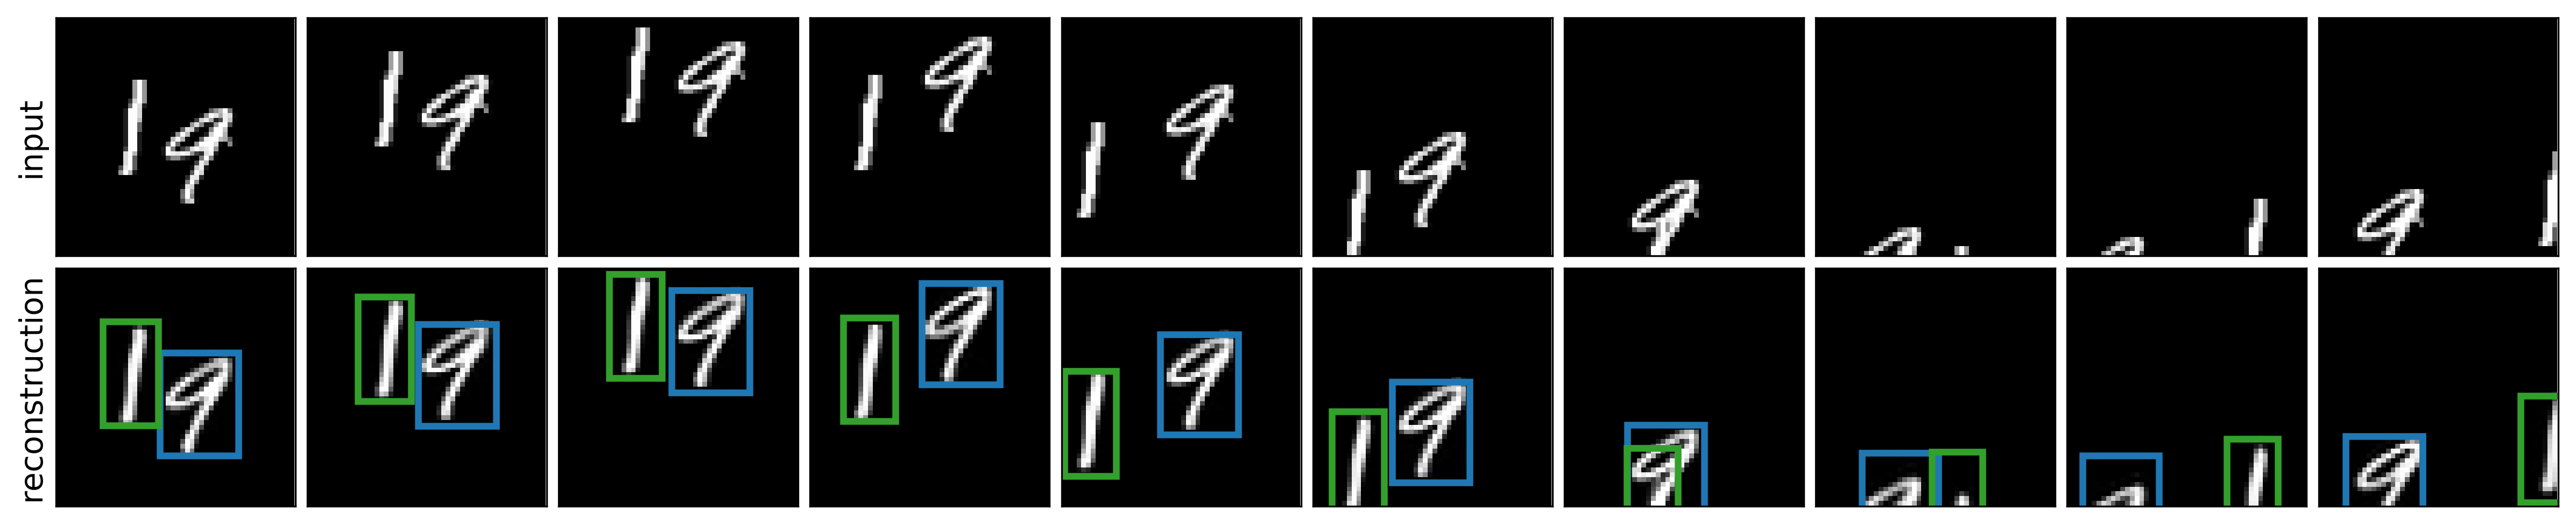
\includegraphics[width=\linewidth]{figures/SQAIR/mnist_rec/000070.png}
    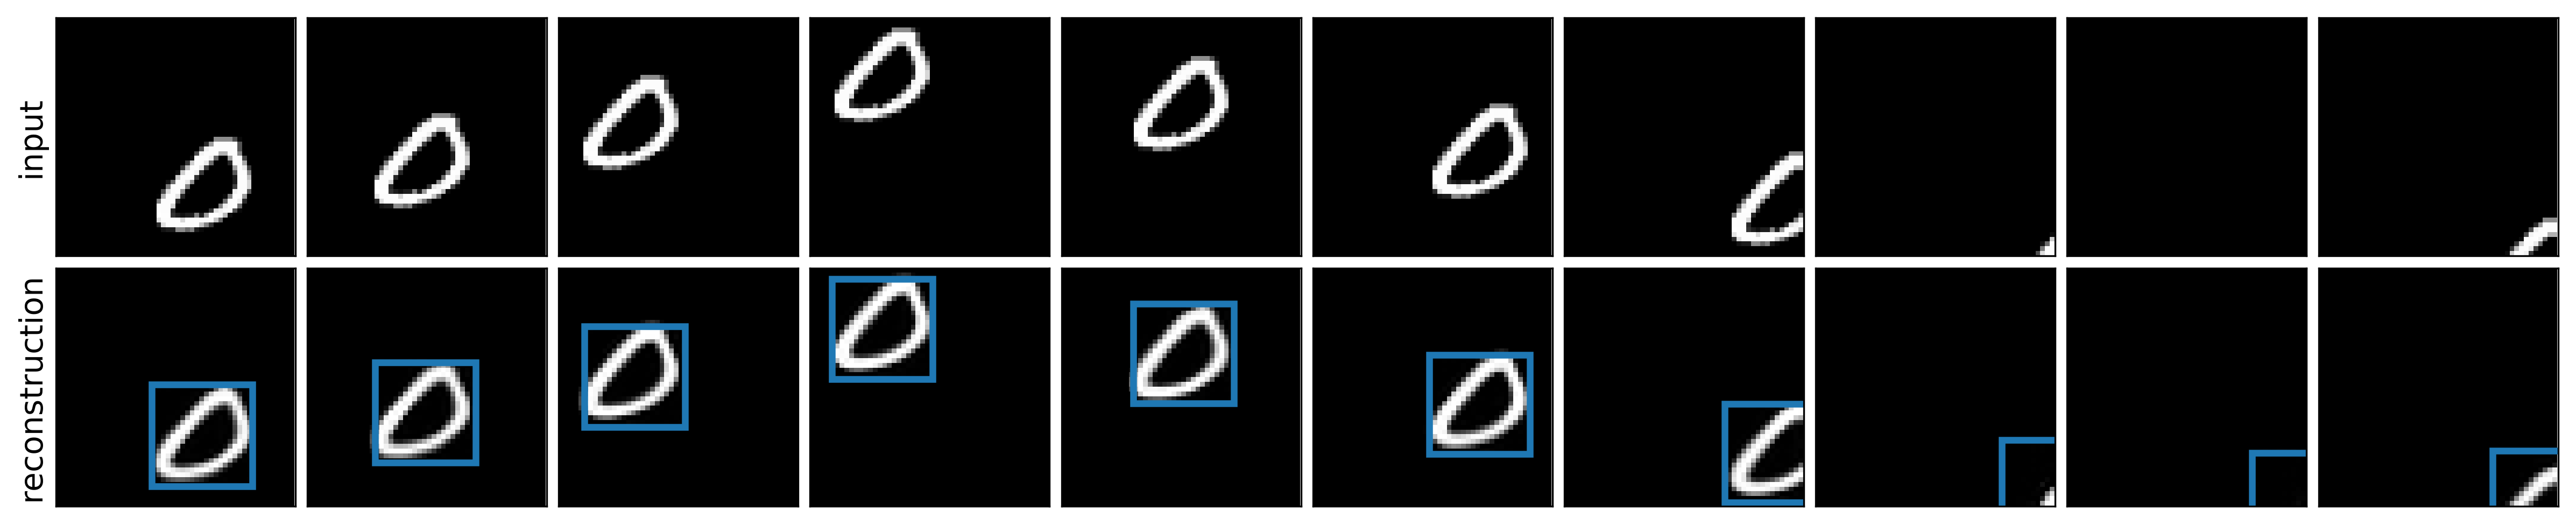
\includegraphics[width=\linewidth]{figures/SQAIR/mnist_rec/000074.png}
    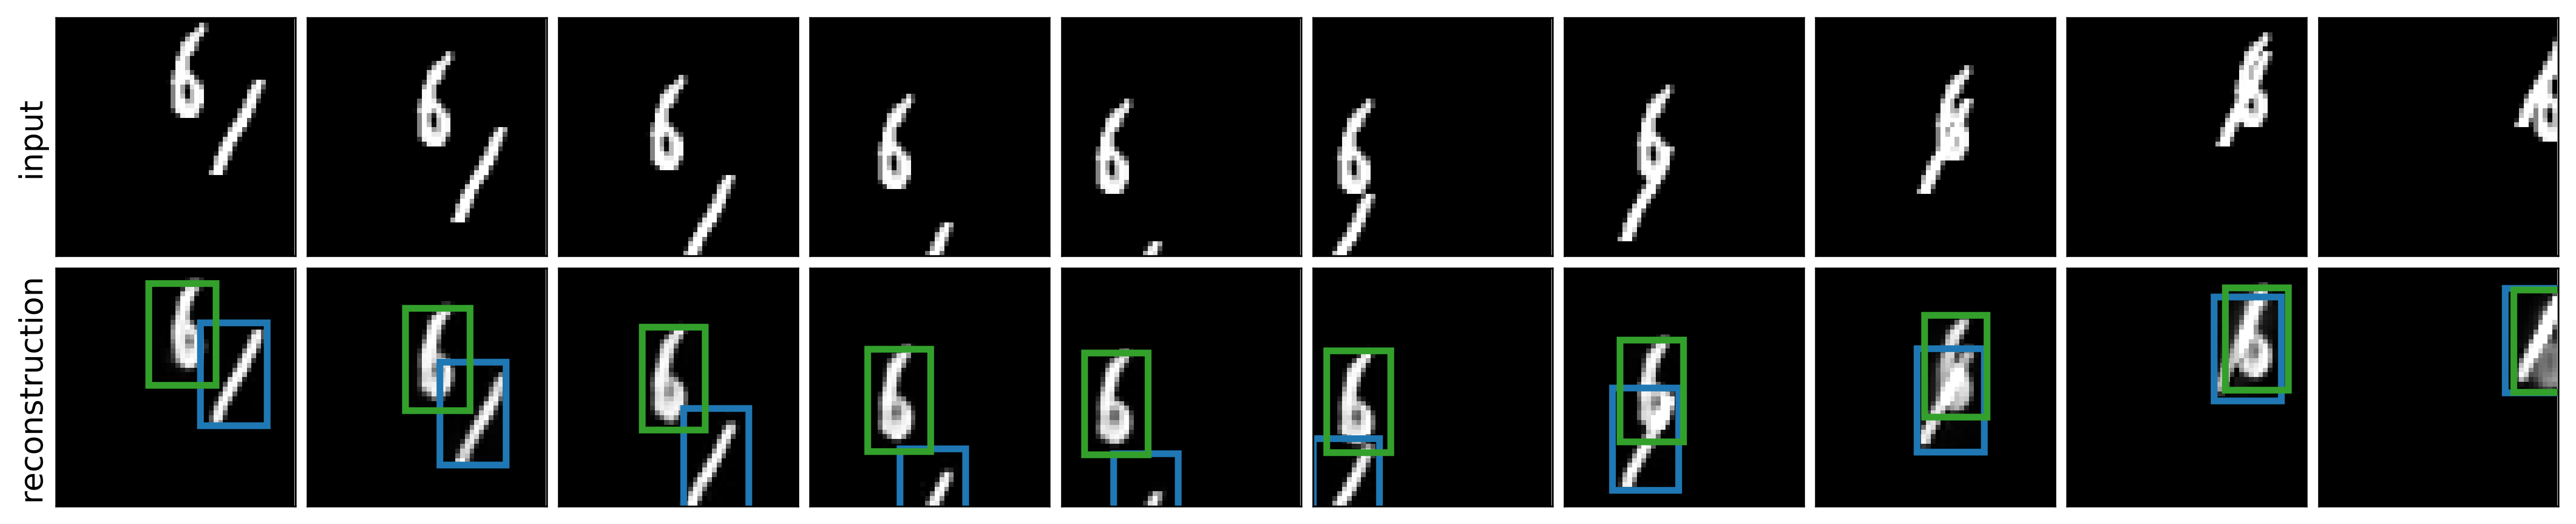
\includegraphics[width=\linewidth]{figures/SQAIR/mnist_rec/000087.png}
    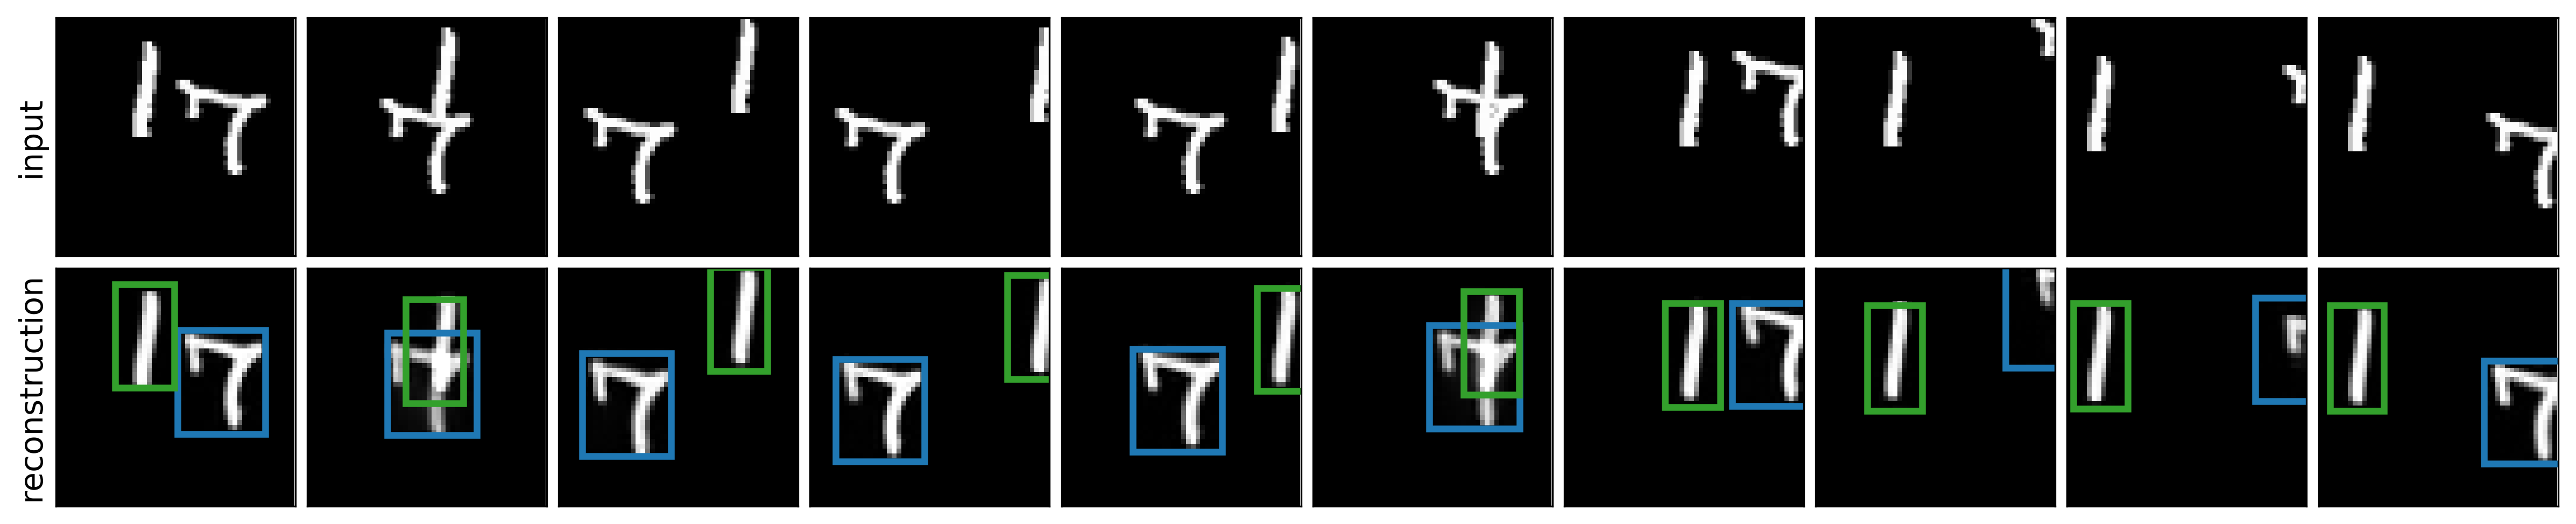
\includegraphics[width=\linewidth]{figures/SQAIR/mnist_rec/000088.png}
    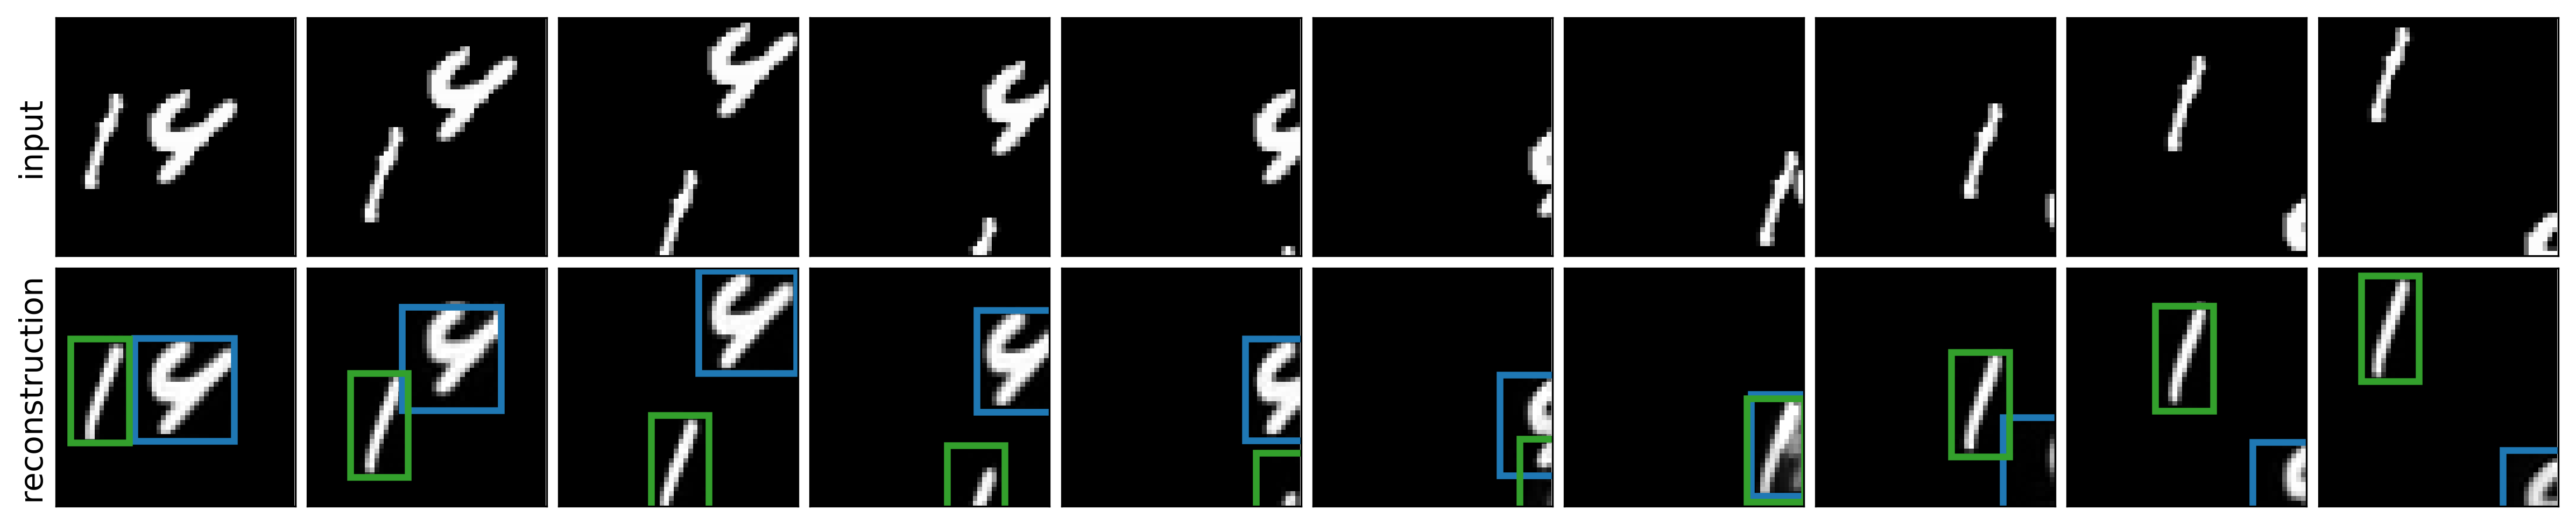
\includegraphics[width=\linewidth]{figures/SQAIR/mnist_rec/000098.png} 
    \captionof{figure}{Sequences of input (first row) and \gls{SQAIR} reconstructions with marked glimpse locations. Reconstructions are all temporally consistent.}
    \label{fig:mnist_recs_additional}
\end{center}




\begin{center}
    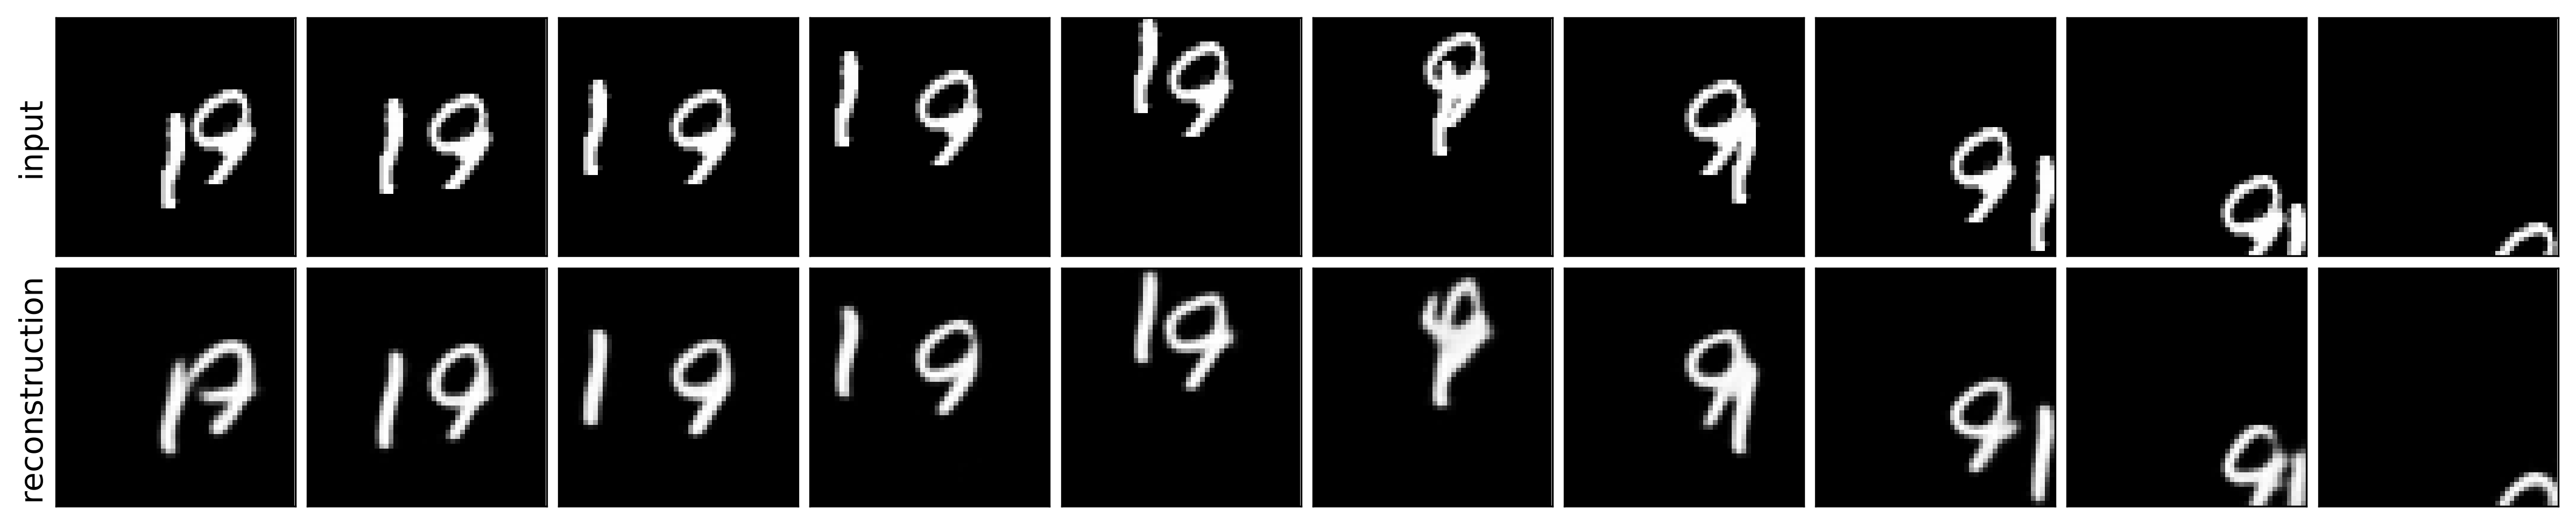
\includegraphics[width=\linewidth]{figures/SQAIR/vrnn_rec/000009.png}
    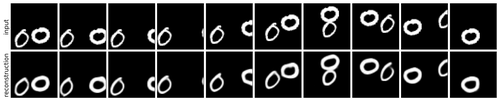
\includegraphics[width=\linewidth]{figures/SQAIR/vrnn_rec/000015.png}
    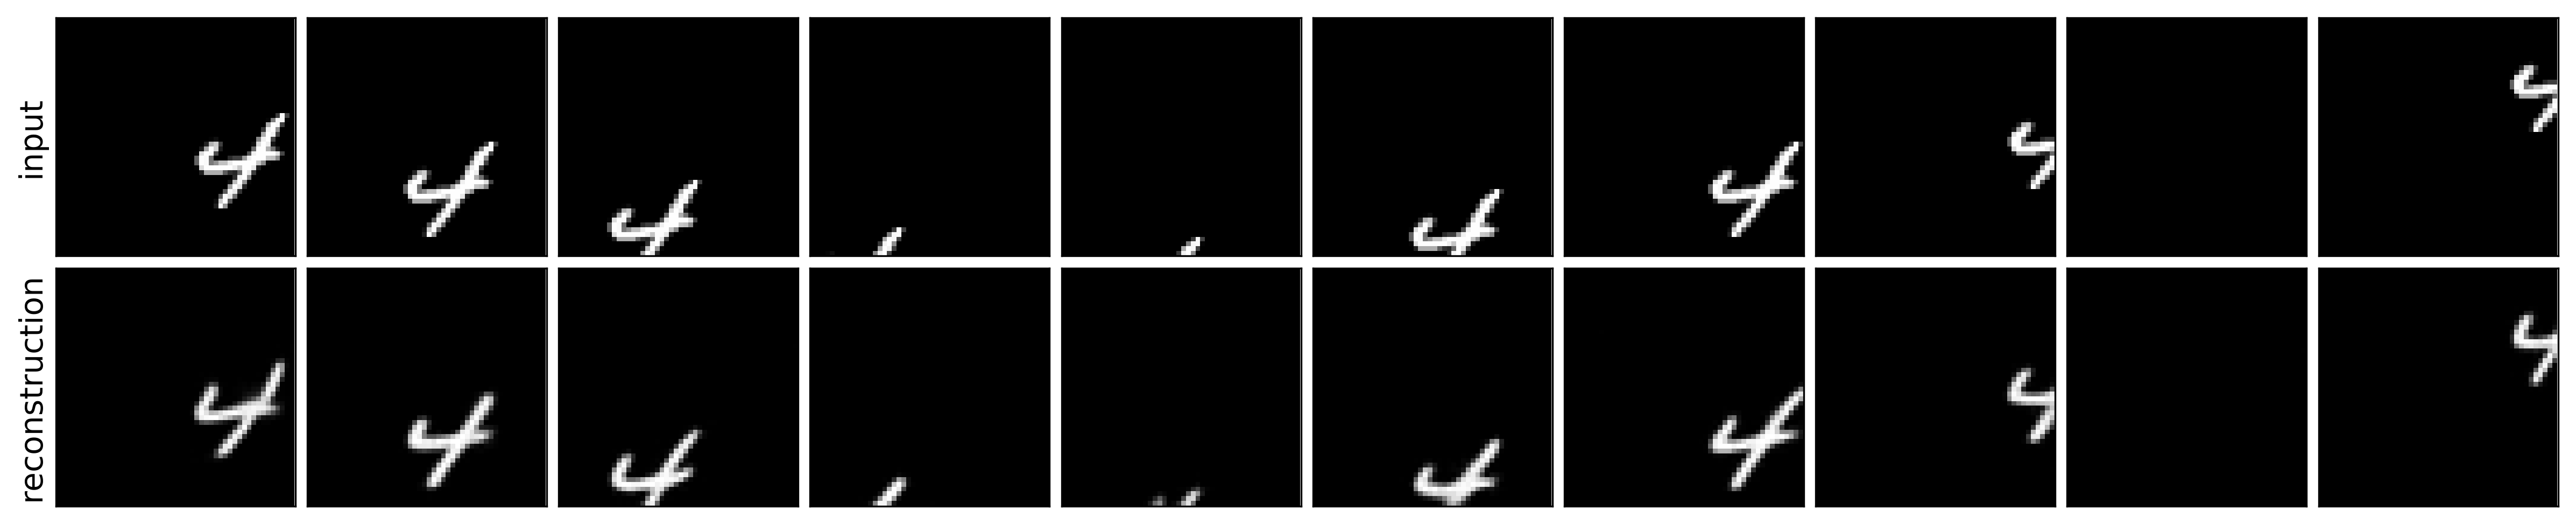
\includegraphics[width=\linewidth]{figures/SQAIR/vrnn_rec/000018.png}
    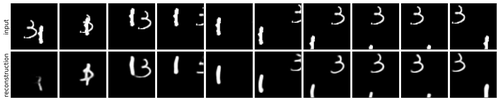
\includegraphics[width=\linewidth]{figures/SQAIR/vrnn_rec/000038.png}
    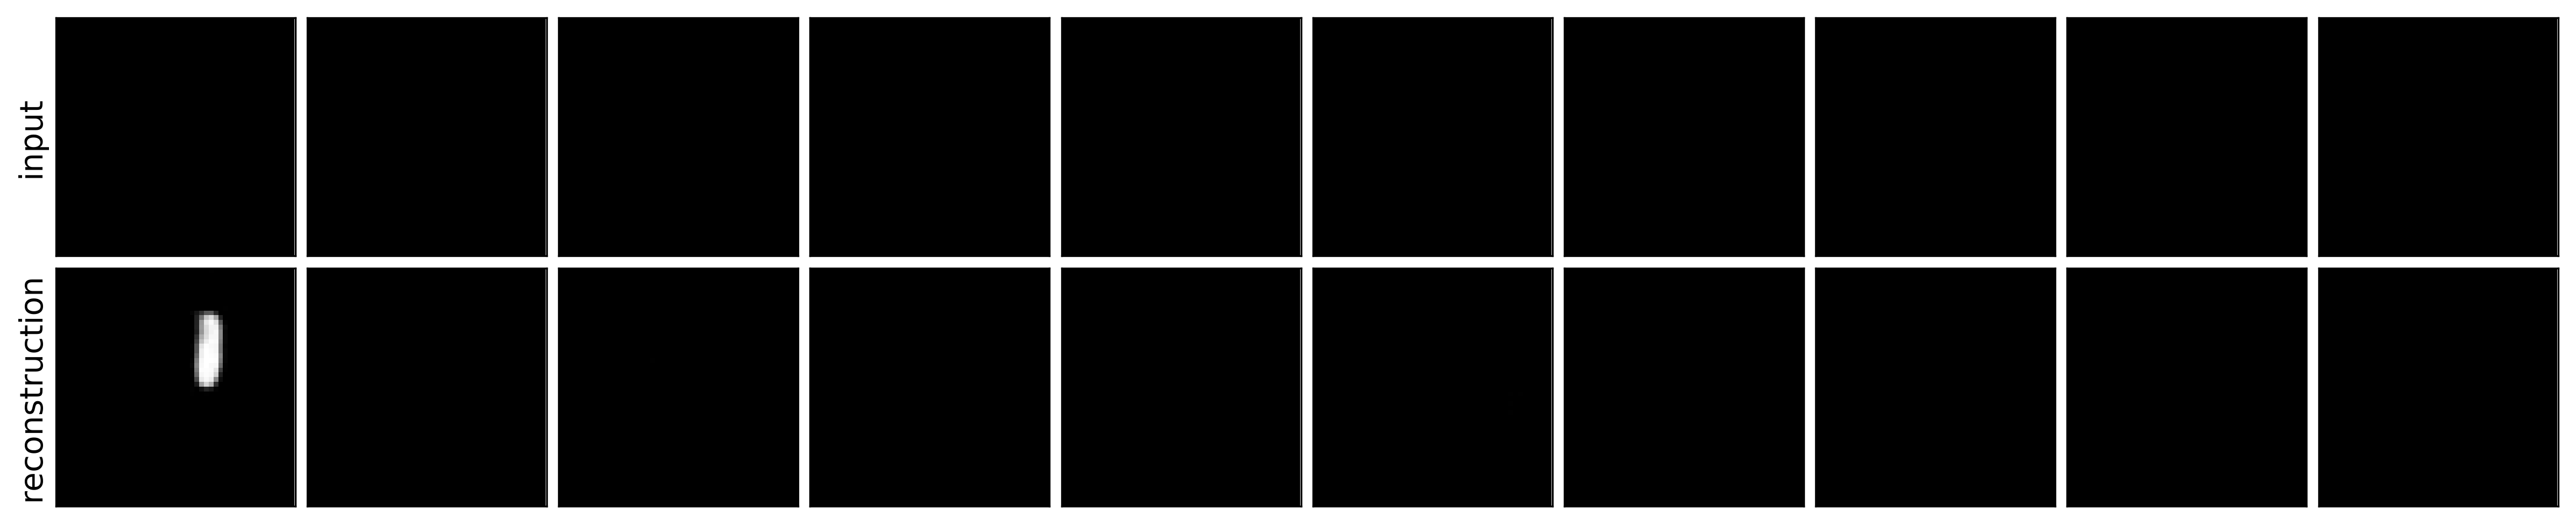
\includegraphics[width=\linewidth]{figures/SQAIR/vrnn_rec/000041.png}
    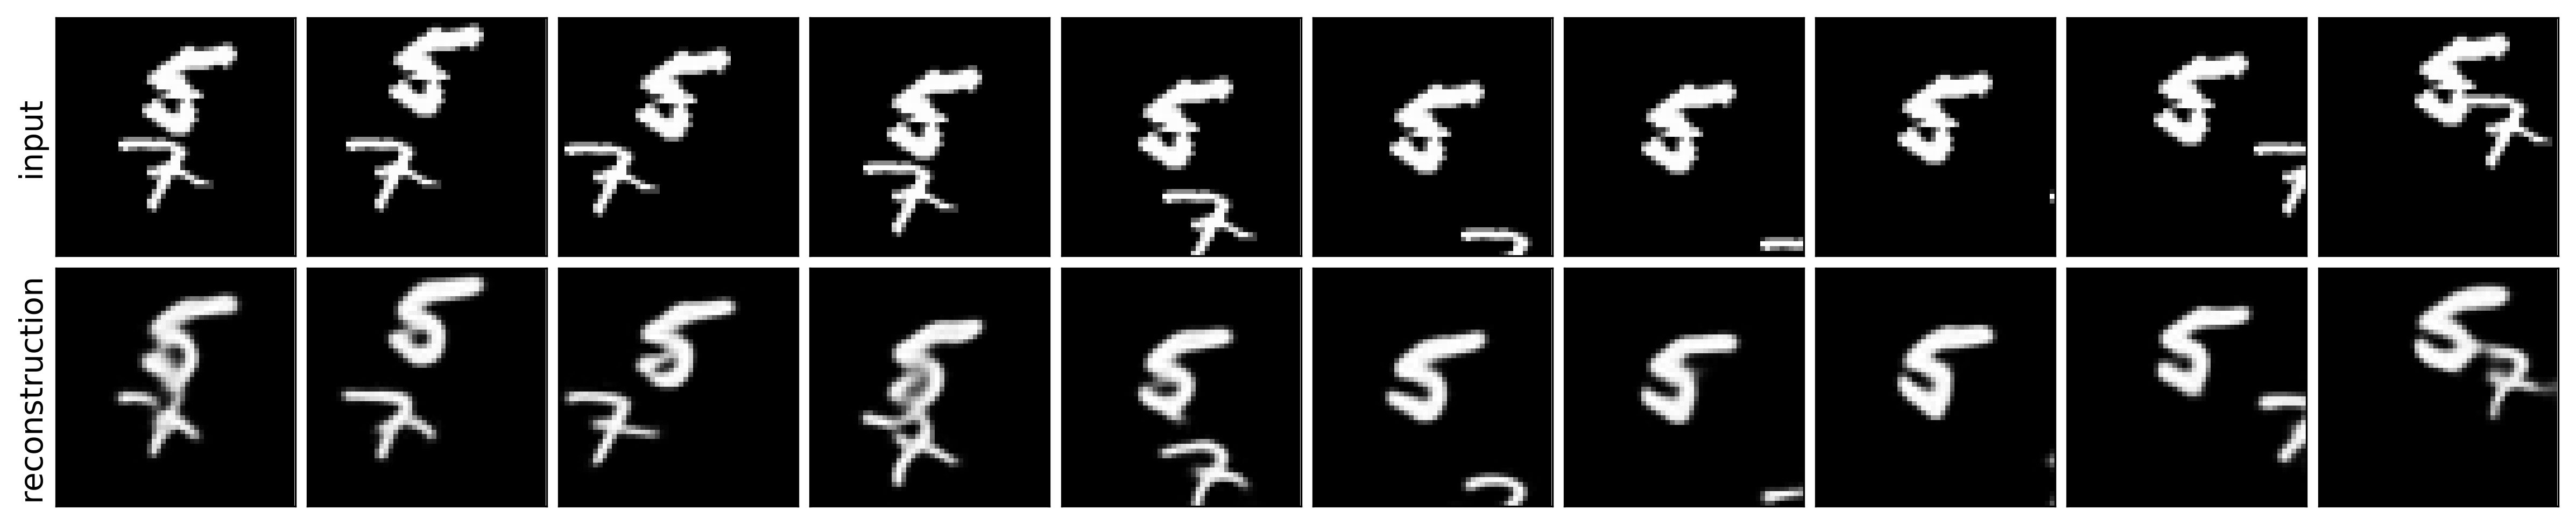
\includegraphics[width=\linewidth]{figures/SQAIR/vrnn_rec/000050.png}
    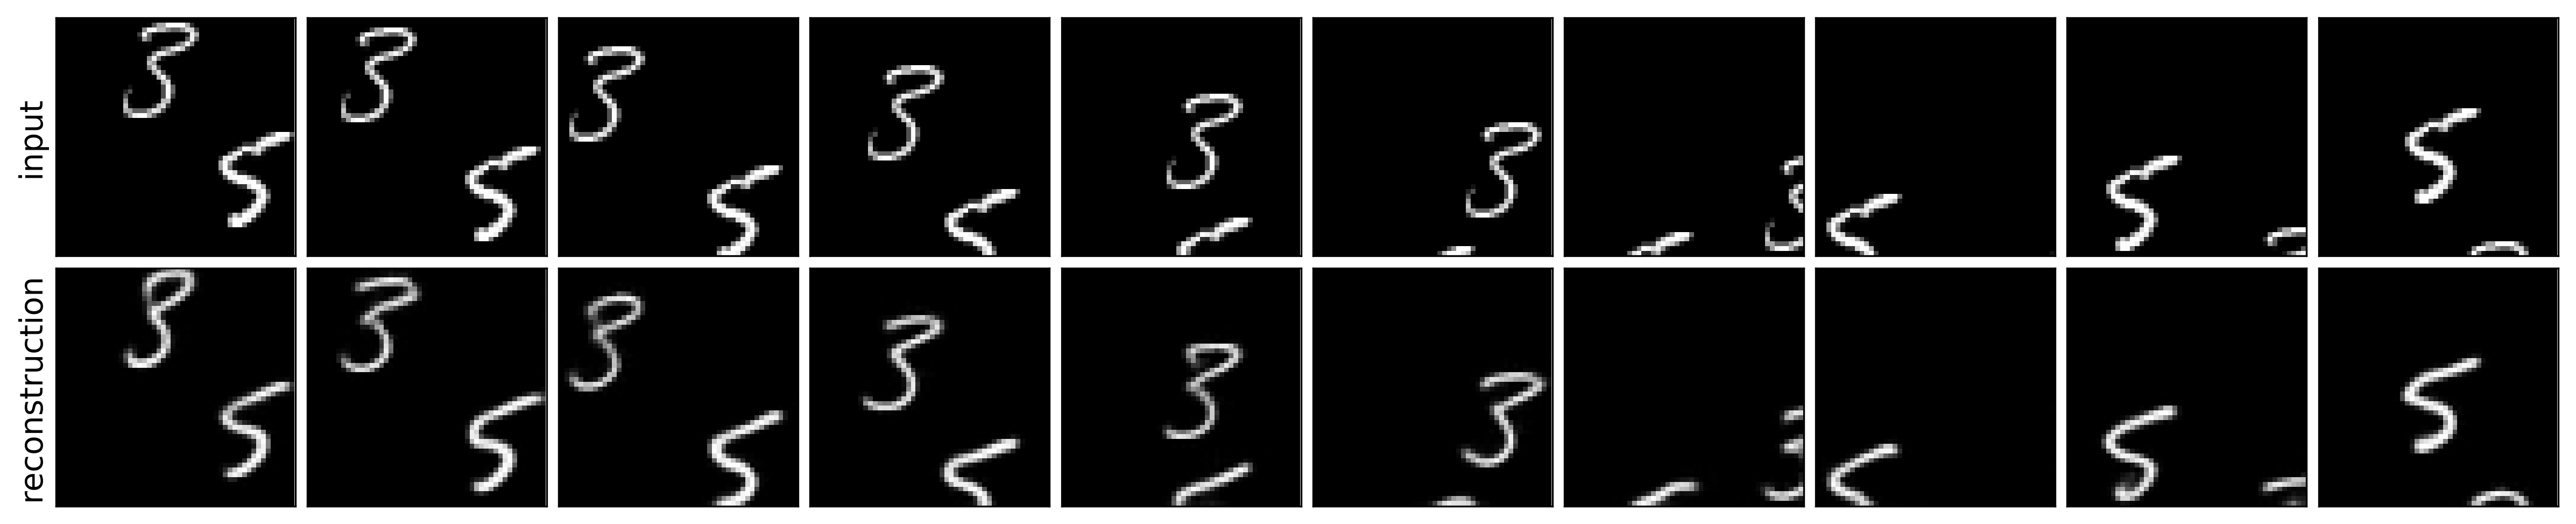
\includegraphics[width=\linewidth]{figures/SQAIR/vrnn_rec/000066.png}
    \captionof{figure}{Sequences of input (first row) and \textsc{conv}-\gls{VRNN} reconstructions. They are not temporally consistent. The reconstruction at time $t=1$ is typically of lower quality and often different than the rest of the sequence.}
    \label{fig:mnist_recs_vrnn}
\end{center}

\subsection{Samples}
\begin{center}
    
\includegraphics[width=\linewidth]{figures/SQAIR/mnist_samples/000044.png}
    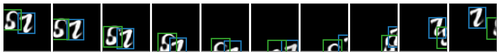
\includegraphics[width=\linewidth]{figures/SQAIR/mnist_samples/000059.png}
    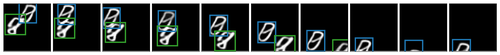
\includegraphics[width=\linewidth]{figures/SQAIR/mnist_samples/000060.png}
    
\includegraphics[width=\linewidth]{figures/SQAIR/mnist_samples/000062.png}
    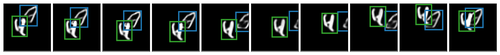
\includegraphics[width=\linewidth]{figures/SQAIR/mnist_samples/000071.png}
    
\includegraphics[width=\linewidth]{figures/SQAIR/mnist_samples/000073.png}
    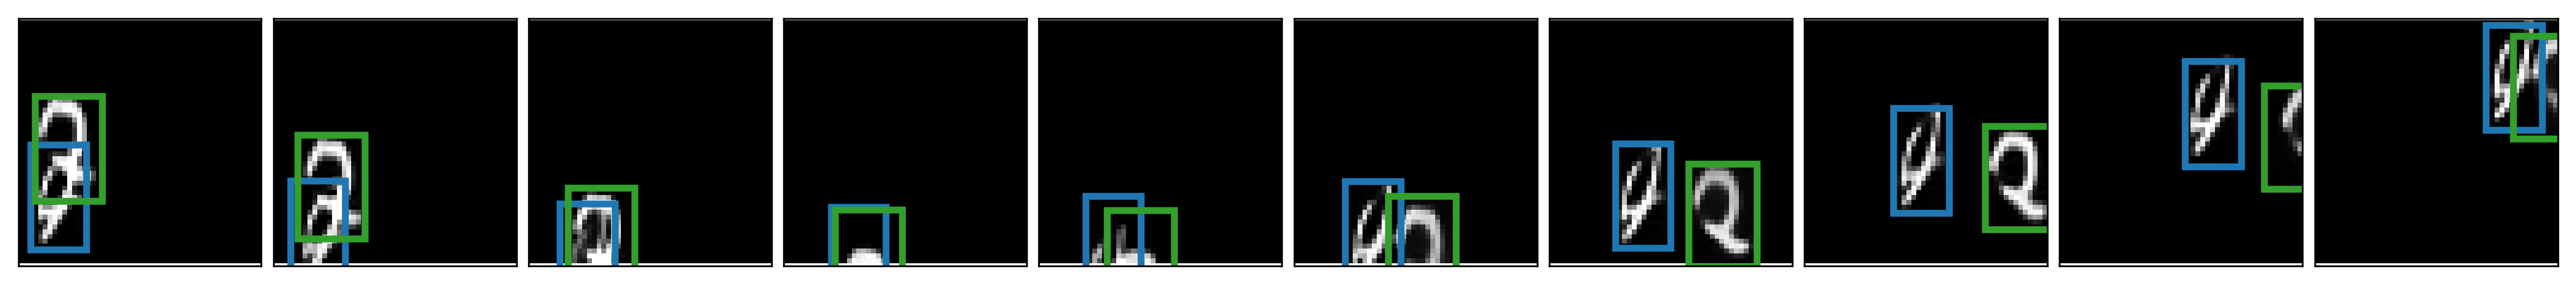
\includegraphics[width=\linewidth]{figures/SQAIR/mnist_samples/000092.png}
    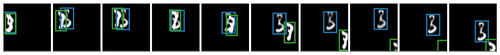
\includegraphics[width=\linewidth]{figures/SQAIR/mnist_samples/000157.png}
    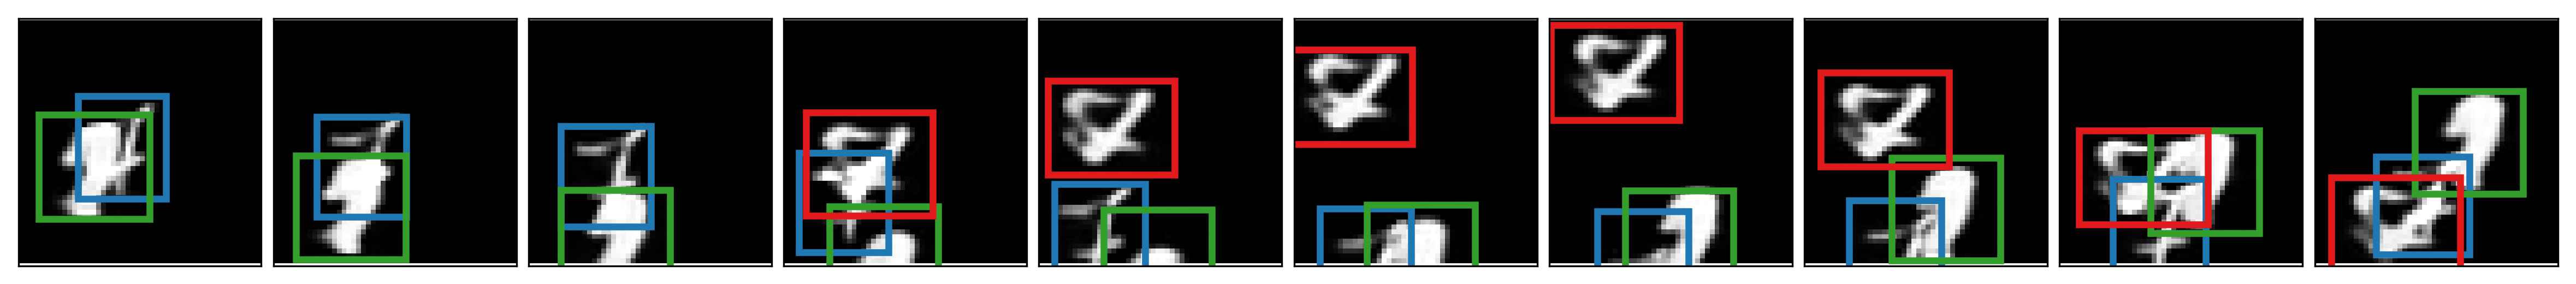
\includegraphics[width=\linewidth]{figures/SQAIR/mnist_sample_curious/000089.png}
    \captionof{figure}{Samples from \gls{SQAIR}. Both motion and appearance are temporally consistent. In the last sample, the model introduces the third object despite the fact that it has seen only up to two objects in training.}
    \label{fig:mnist_samples_additional}
\end{center}


\newpage
\begin{center}
    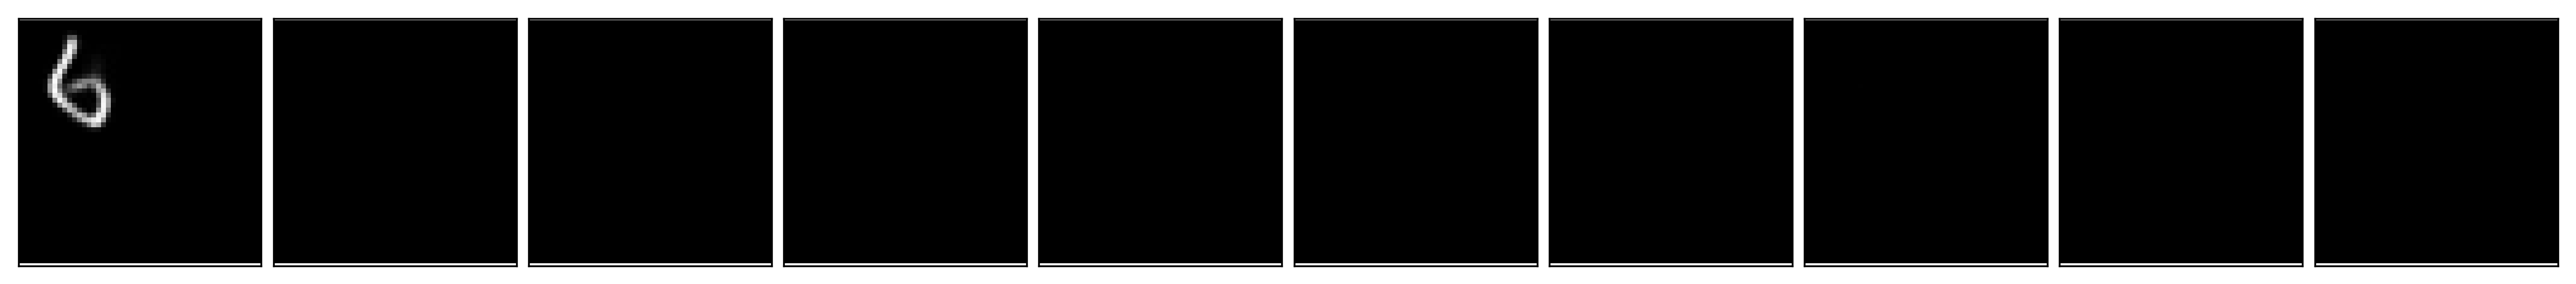
\includegraphics[width=\linewidth]{figures/SQAIR/vrnn_samples/000002.png}
    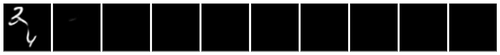
\includegraphics[width=\linewidth]{figures/SQAIR/vrnn_samples/000004.png}
    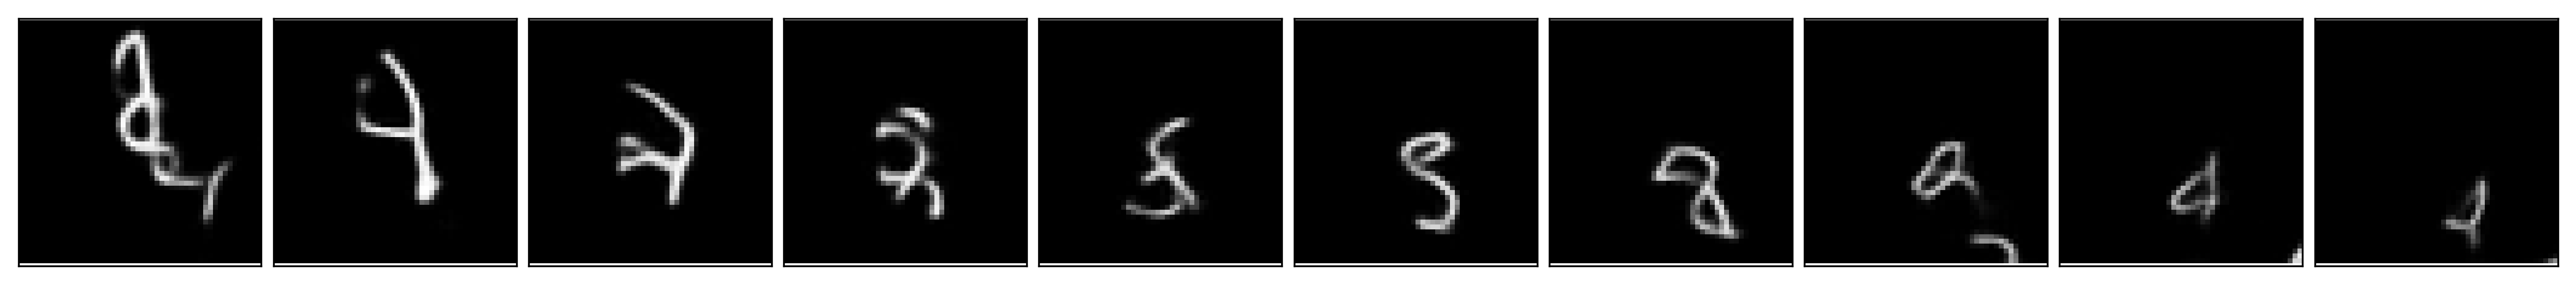
\includegraphics[width=\linewidth]{figures/SQAIR/vrnn_samples/000007.png}
    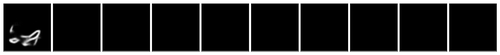
\includegraphics[width=\linewidth]{figures/SQAIR/vrnn_samples/000009.png}
    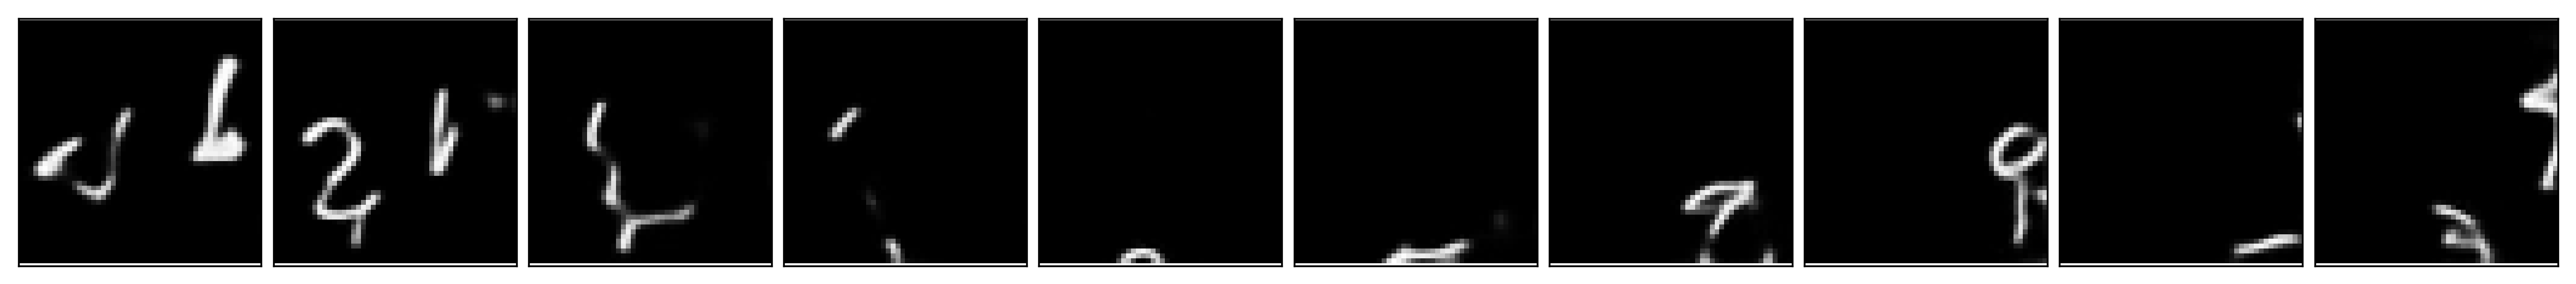
\includegraphics[width=\linewidth]{figures/SQAIR/vrnn_samples/000012.png}
    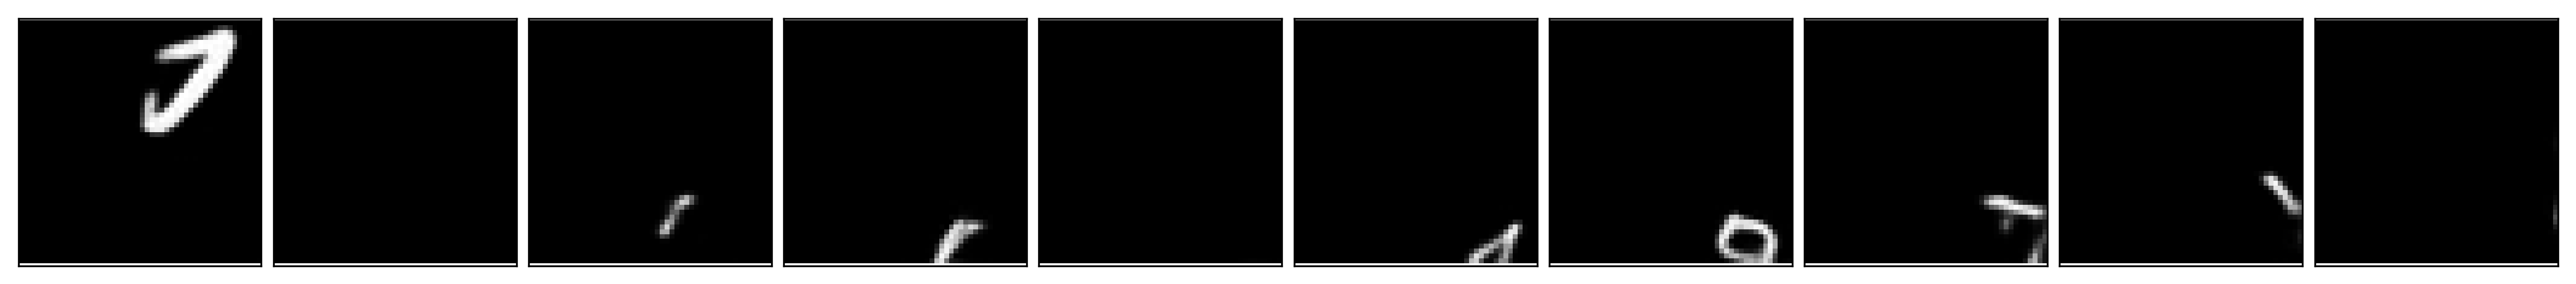
\includegraphics[width=\linewidth]{figures/SQAIR/vrnn_samples/000013.png}
    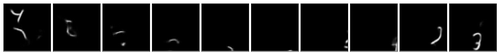
\includegraphics[width=\linewidth]{figures/SQAIR/vrnn_samples/000016.png}
    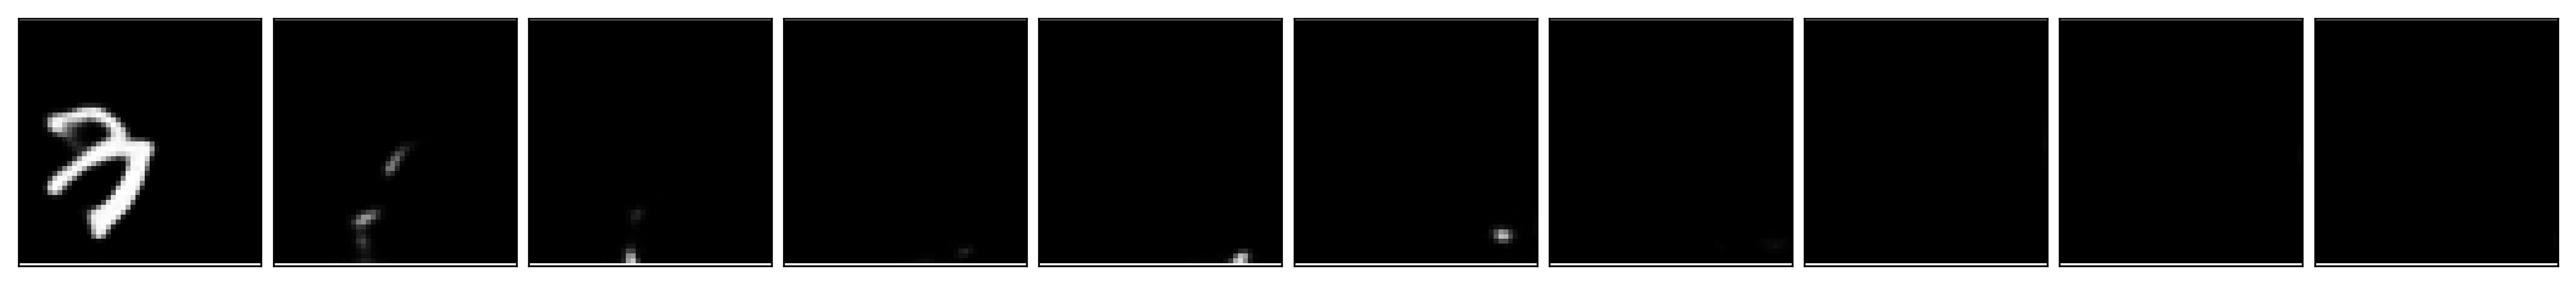
\includegraphics[width=\linewidth]{figures/SQAIR/vrnn_samples/000066.png}
    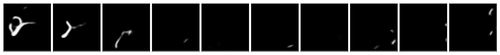
\includegraphics[width=\linewidth]{figures/SQAIR/vrnn_samples/000084.png}
    \captionof{figure}{Samples from \textsc{conv}-\gls{VRNN}. They show lack of temporal consistency. Objects in the generated frames change between consecutive time-steps and they do not resamble digits from the training set.}
    \label{fig:mnist_samples_vrnn}
\end{center}

\newpage
\subsection{Conditional Generation}

\begin{center}
    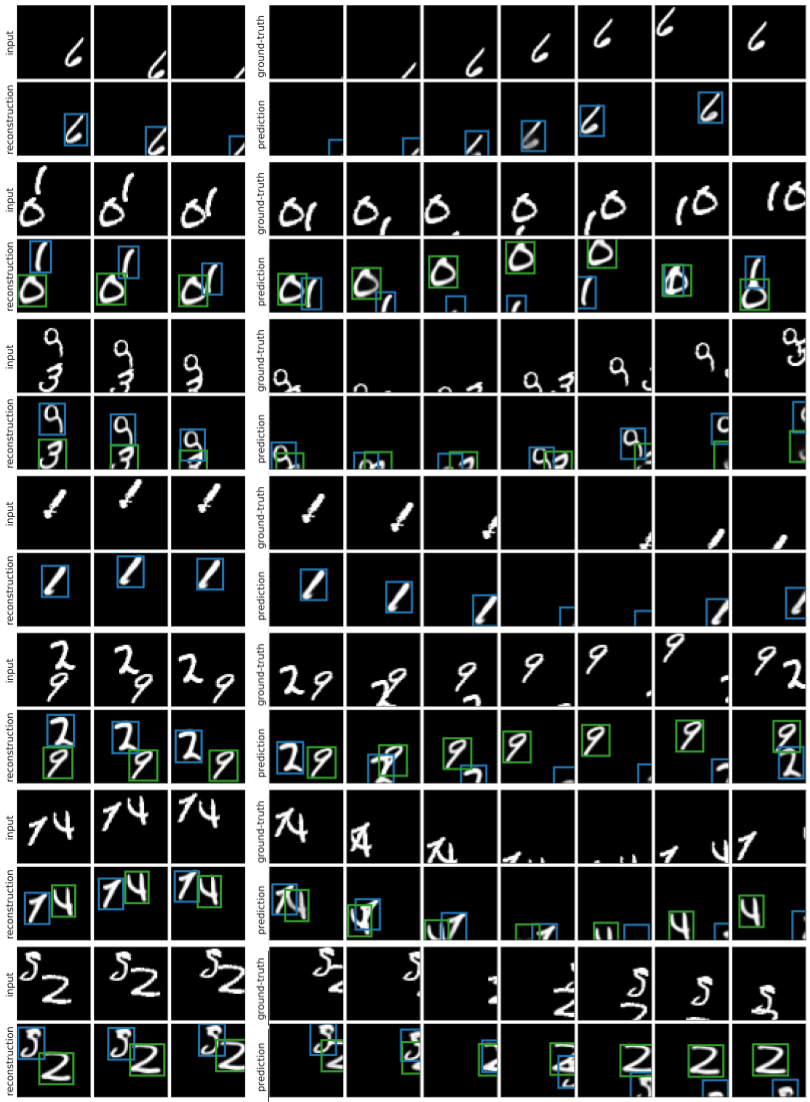
\includegraphics[width=\linewidth]{figures/SQAIR/sqair_mnist_cond_gen_appendix}
    \captionof{figure}{Conditional generation from \gls{SQAIR}, which sees only the first three frames in every case. Top is the input sequence (and the remaining ground-truth), while bottom is reconstruction (first three time-steps) and then generation.}
    \label{fig:mnist_cond_gen_sqair}
\end{center}